\documentclass{beamer}
\mode<presentation>
\usetheme{CambridgeUS}
\usepackage[russian]{babel}
\usepackage[utf8]{inputenc}
\usepackage[T2A]{fontenc}
\usepackage{sansmathaccent}

\usepackage{verbatim}
\usepackage{alltt}

\pdfmapfile{+sansmathaccent.map}
\title[Artifical Intelligence]{Кластерный анализ}
\author{Наумов Д.А., доц. каф. КТ}
\date[04.12.2019] {Экспертные системы и искусственный интеллект, 2019}

\begin{document}

%ТИТУЛЬНЫЙ СЛАЙД
\begin{frame}
  \titlepage
\end{frame}
  
%СОДЕРЖАНИЕ ЛЕКЦИИ
\begin{frame}
  \frametitle{Содержание лекции}
  \tableofcontents  
\end{frame}

\section{Кластерный анализ. Основные понятия}

\begin{frame}{Кластеризация}
\begin{block}{Задача кластеризации}
частично сгруппированные точки на плоскости или в пространстве большей размерности разбиваются на близкорасположенные группы.
\end{block}
\begin{figure}[h]
\centering
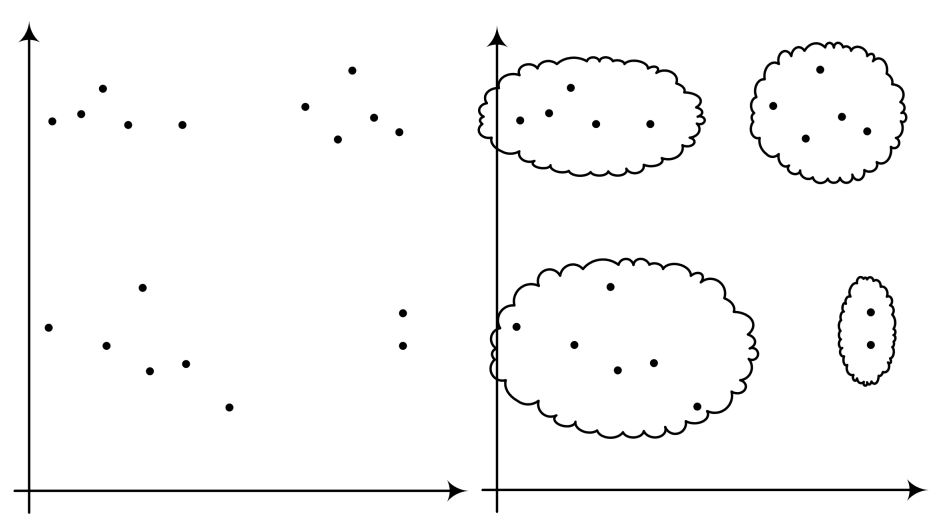
\includegraphics[scale=0.4]{images/lec07-pic01.png}
\end{figure}
\end{frame}

\begin{frame}{Кластеризация}
\begin{figure}[h]
\centering
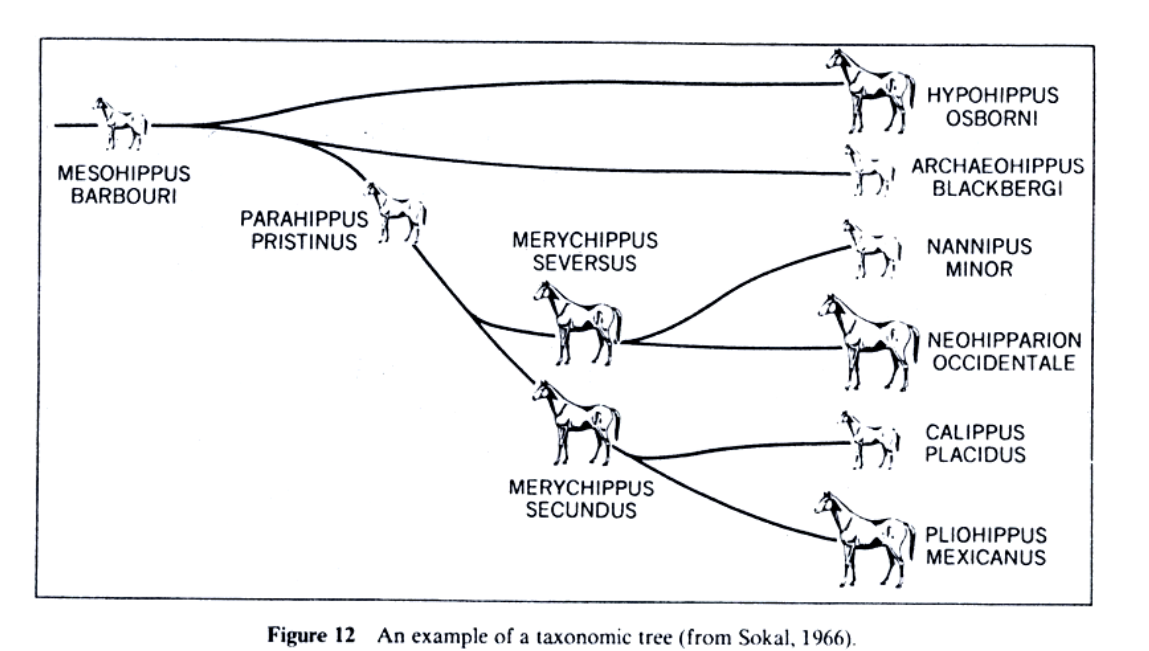
\includegraphics[scale=0.4]{images/lec07-pic06.png}
\end{figure}
\end{frame}

\begin{frame}{Задачи кластеризации}
\begin{itemize}
\item лежат в основе анализа данных (data mining);
	\begin{itemize}
	\item анализ покупок в супермаркетах;
	\item разделение документов на жанры и тематики;
	\item контекстная рекалама и анализ предпочтений пользователя.	
	\end{itemize}
\item распознование образов: получение границ областей и выделение общих принаков;
\item биоинформатика: анализ длинных последовательностей атомов в белках 	
	\begin{itemize}
	\item разбиение генов на кластеры;
	\item выделение генов на группы по функциональной схожести;
	\item выделение генов, отвечающие за биологическое свойство.	
	\end{itemize}
\item маркетологические исследования для сегментации рынка;	
\item анализ социальныз сетей;
\end{itemize}
\end{frame}

\begin{frame}{Кластеризация}
\begin{block}{Кластеризация - типичная задача статистического анализа}
задача классификации объектов одной природы в несколько групп так, чтобы объекта одной группы обладали
одним и тем же свойством. Под свойством понимается близоть друг к другу относительно выбранной метрики.
\end{block}
Сложность задачи кластеризации:
\begin{itemize}
\item высокая размерность реальных задач (сотни и тысячи);
\item необхождим компромис: число точек и размерность пространства.
\end{itemize}
\end{frame}

\begin{frame}
\begin{minipage}{0.4\textwidth}
\begin{flushleft}
\begin{figure}[h]
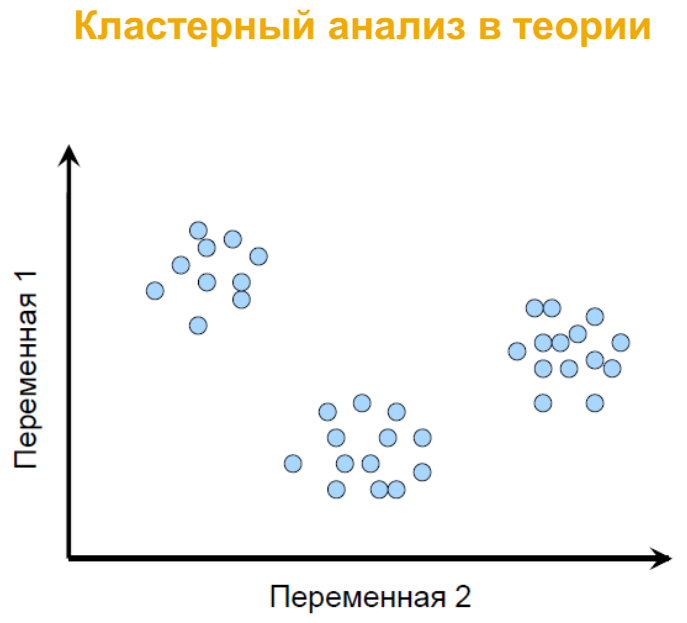
\includegraphics[scale=0.3]{images/lec07-pic04.png}
\end{figure}
\end{flushleft}
\end{minipage}
\hfill
\begin{minipage}{0.5\textwidth}
\begin{flushright}
\begin{figure}[h]
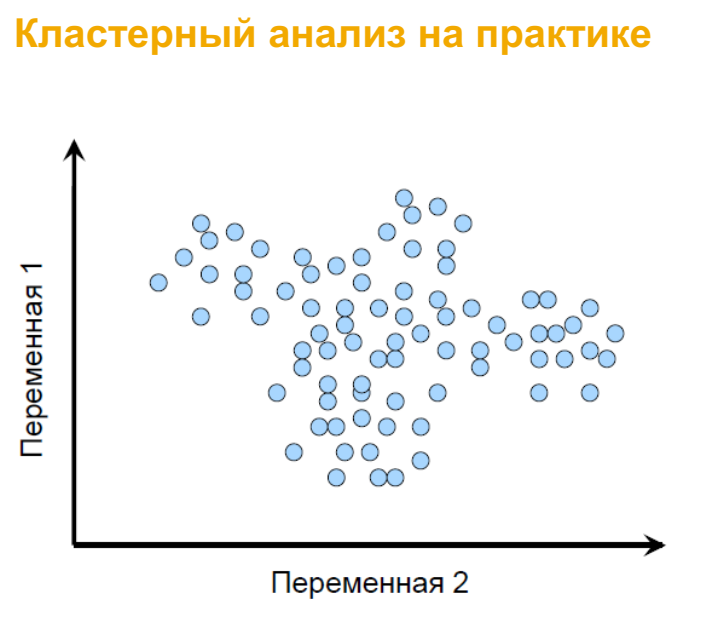
\includegraphics[scale=0.3]{images/lec07-pic05.png}
\end{figure}
\end{flushright}
\end{minipage}
\end{frame}

\begin{frame}{Кластеризация}
Пусть дан набор тестовых примеров
\begin{figure}[h]
\centering
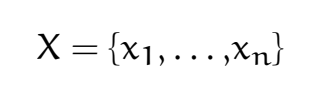
\includegraphics[scale=0.4]{images/lec07-pic02.png}
\end{figure}
и функция расстояния между ними
\begin{figure}[h]
\centering
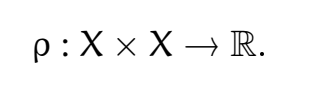
\includegraphics[scale=0.4]{images/lec07-pic03.png}
\end{figure}
Требуется разбить X на непересекающиеся подмножества, которые, собственно, и называются кластерами, так, чтобы каждое подмножество состояло из \textit{близких объектов}, а объекты разных подмножеств \textit{существенно различались}.
\begin{itemize}
\item что такое "близкие объекты"?
\item что такое "существенно различающиеся объекты"?
\end{itemize}
\end{frame}

\begin{frame}{Меры близости между объектами}
\begin{figure}[h]
\centering
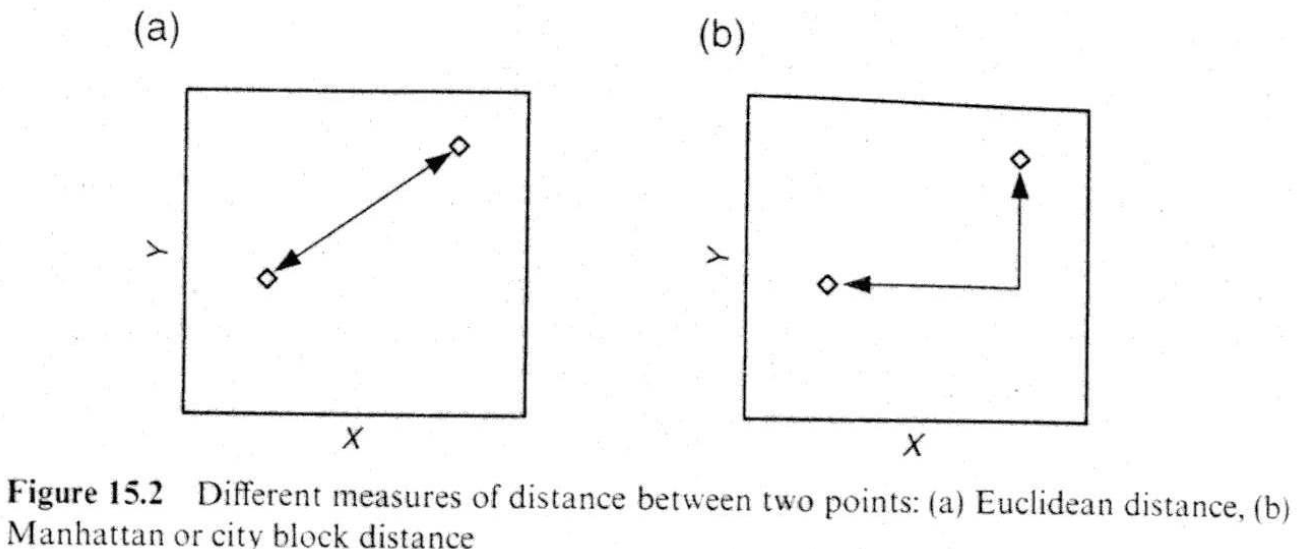
\includegraphics[scale=0.3]{images/lec07-pic07.png}
\end{figure}
\end{frame}

\begin{frame}{Меры близости между объектами}
\begin{figure}[h]
\centering
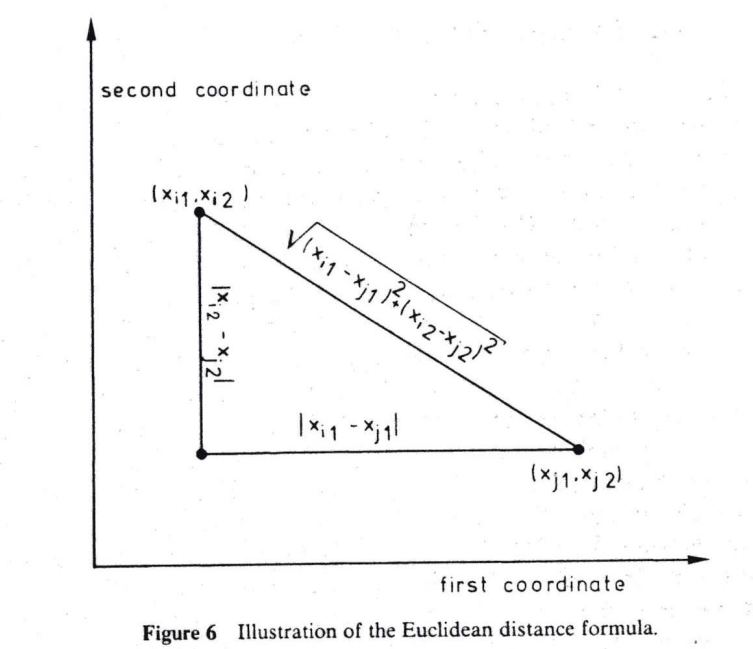
\includegraphics[scale=0.4]{images/lec07-pic08.png}
\end{figure}
\end{frame}

\begin{frame}{Меры близости между объектами}
\begin{figure}[h]
\centering
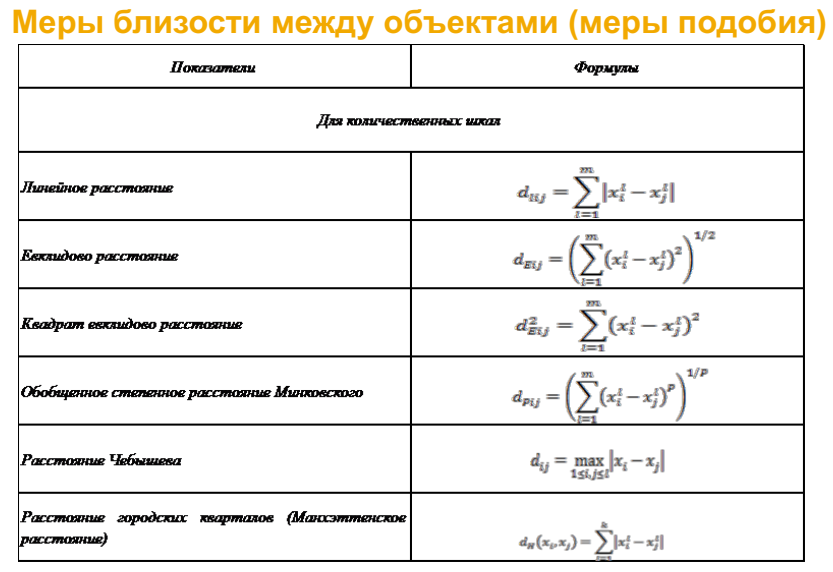
\includegraphics[scale=0.4]{images/lec07-pic09.png}
\end{figure}
\end{frame}

\begin{frame}{Расстояние tf-idf}
\begin{block}{tf-idf}
мера близости двух текстовых документов
\end{block}
Документ представляется в виде вектора из $n$ термов с некоторыми весами. Разные подходы к анализу текстов различаются в том:  
\begin{itemize}
\item что такое терм;
\item как определять веса.
\end{itemize}
\begin{block}{Термы}
(обычно) слова, встречающиеся в документе. 
\end{block}
Документ превращается при этом в неупорядоченный набор слов (bag of words).

Cложные структуры в качестве термов? нецелесообразно!
\begin{itemize}
\item нужно будет слишком много текстов, 
\item результат не будет существенно лучше bag-of-words подхода.
\end{itemize}  
\end{frame}

\begin{frame}{Расстояние tf-idf}
Для определения весов обычно используют два основных подхода:
\begin{itemize}
\item либо бинарный атрибут со значениями 01 (есть слово или нет слова),
\item либо весовую функцию, меру tdf (term frequency  inverse document frequency).
\end{itemize}  

\begin{block}{Мера tf-idf}
\begin{itemize}
\item была предложена в начале 1970-х годов и с тех пор активно используется в анализе текстовой информации и information retrieval;
\item состоит из двух других: tf (частота терма, term frequency) и idf (обратная частота
терма в документах, inverse document frequency).
\end{itemize}
\end{block}
\end{frame}

\begin{frame}{Расстояние tf-idf}
\begin{block}{Частота терма}
доля числа появлений этого терма по отношению к размеру всего документа.
\end{block}
\begin{figure}[h]
\centering
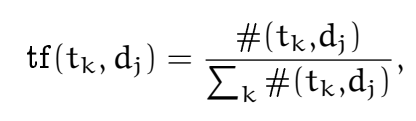
\includegraphics[scale=0.4]{images/lec07-pic10.png}
\end{figure}
где \#(tk,dj) - число, показывающее, сколько раз терм tk встречается в документе dj.
\end{frame}

\begin{frame}{Расстояние tf-idf}
\begin{block}{Обратная частота терма}
показывает, насколько терм вообще важен, насколько он характерен для данного массива текстов.
\end{block}
Чем реже встречается терм в имеющемся массиве, тем он характернее.
\begin{figure}[h]
\centering
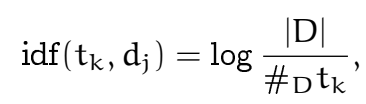
\includegraphics[scale=0.4]{images/lec07-pic11.png}
\end{figure}
где где D - имеющийся набор данных, а \#Dtk - количество документов из D, в которых хотя бы однажды встречается tk.
\end{frame}

\begin{frame}{Расстояние tf-idf}
Мера tdf для терма tk и документа dj в массиве D равна:
\begin{figure}[h]
\centering
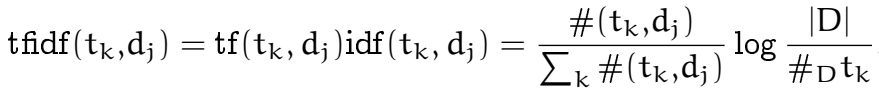
\includegraphics[scale=0.4]{images/lec07-pic12.png}
\end{figure}
Вектор весом можно нормализовать:
\begin{figure}[h]
\centering
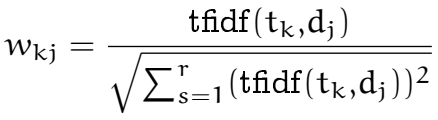
\includegraphics[scale=0.4]{images/lec07-pic13.png}
\end{figure}
Теперь документ можно представить в виде вектора, размерность которого равна количеству термов (важно сохранять словарь не слишком большим за счет удачного выбора термов).
\end{frame}

\begin{frame}{Расстояние между документами}
Расстояние между документами - используется не простое декартово расстояние, а угол между векторами, косинусоидальная мера похожести (cosine similarity measure):
\begin{figure}[h]
\centering
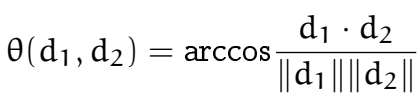
\includegraphics[scale=0.4]{images/lec07-pic14.png}
\end{figure}
\end{frame}

\section{Иерархическая кластеризация}

\begin{frame}{Кластерный анализ}
\begin{figure}[h]
\centering
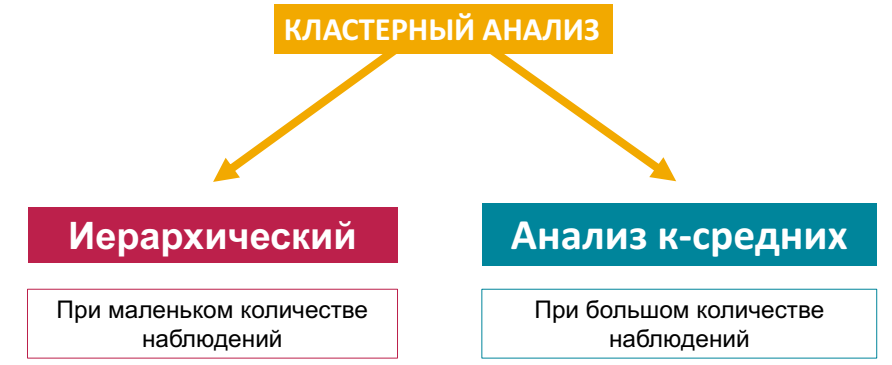
\includegraphics[scale=0.5]{images/lec07-pic15.png}
\end{figure}
\begin{itemize}
\item иерархическая кластеризация - алгоритм последовательно строит кластеры из уже найденных кластеров;
\item неиерархическая кластеризация - алгоритм пытается распознать всю структуру сразу или строит кластеры один за другим, не разделяя и не соединяя уже выделенные кластеры.
\end{itemize}
\end{frame}

\begin{frame}{Кластерный анализ}
Иерархическая кластеризация:
\begin{itemize}
\item агломеративная: алгоритм начинает с индивидуальных элементов (кластеров из одного элемента), а затем последовательно объединяет их, получая требуемую структуру; 
\item разделительная, когда алгоритм начинает с одного кластера, содержащего все точки, а потом последовательно делит его на части.
\end{itemize}
Неиерархические методы, как правило, стремятся оптимизировать некую целевую функцию, которая описывает качество кластеризации. 
\begin{itemize}
\item агоритмы, основанные на методах теории графов;
\item алгоритм EM;
\item алгоритм k-средних;
\item нечеткие алгоритмы.
\end{itemize}
\end{frame}

\begin{frame}
\textbf{Иерархическая кластеризация.} Пусть нужно кластеризовать точки x1,x2, . . . ,xn в некотором метрическом пространстве с метрикой.
\begin{enumerate}
\item на первом шаге мы считаем каждую точку отдельным кластером;
\item ближайшие точки объединяем и далее относимся к ним как к единому кластеру.
\item при итерации этого процесса получается дерево, в листьях которого  отдельные точки, а в корне  кластер, содержащий все точки вообще.
\end{enumerate}
\begin{figure}[h]
\centering
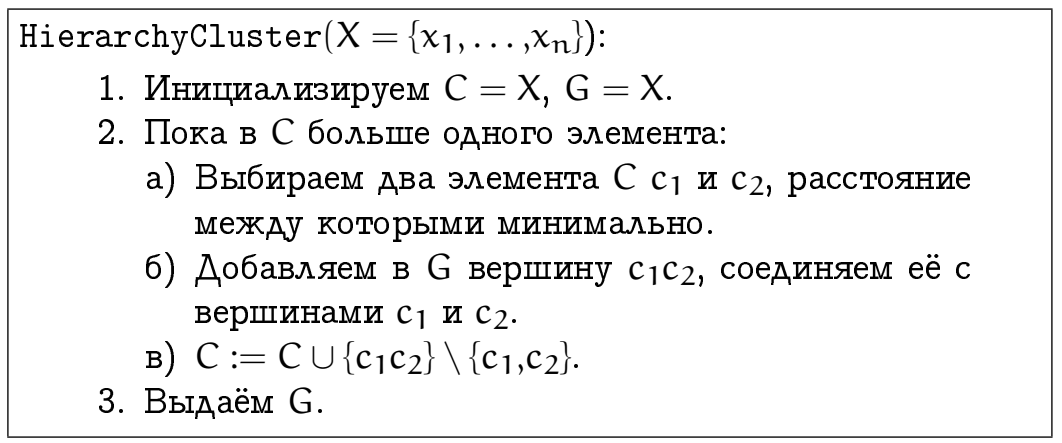
\includegraphics[scale=0.4]{images/lec07-pic16.png}
\end{figure}
\end{frame}

\begin{frame}{Расстояние между кластерами}
\begin{figure}[h]
\centering
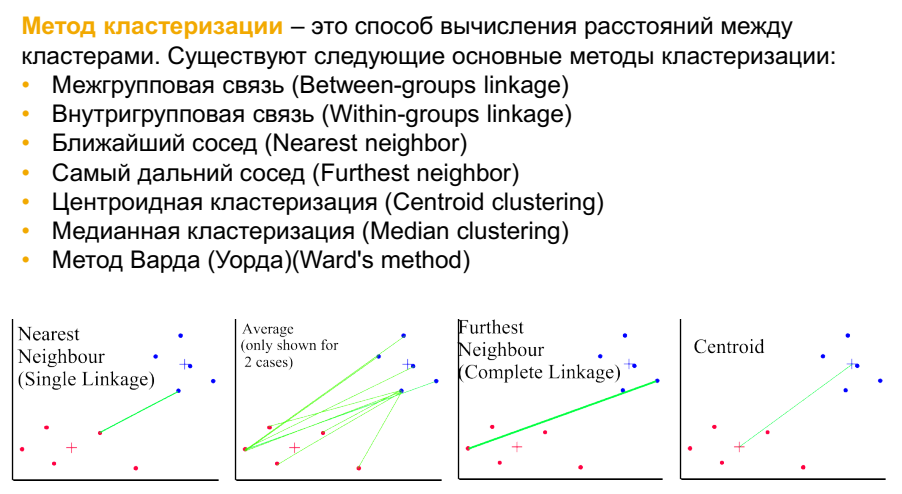
\includegraphics[scale=0.4]{images/lec07-pic17.png}
\end{figure}
\end{frame}

\begin{frame}{Расстояние между кластерами}
\begin{figure}[h]
\centering
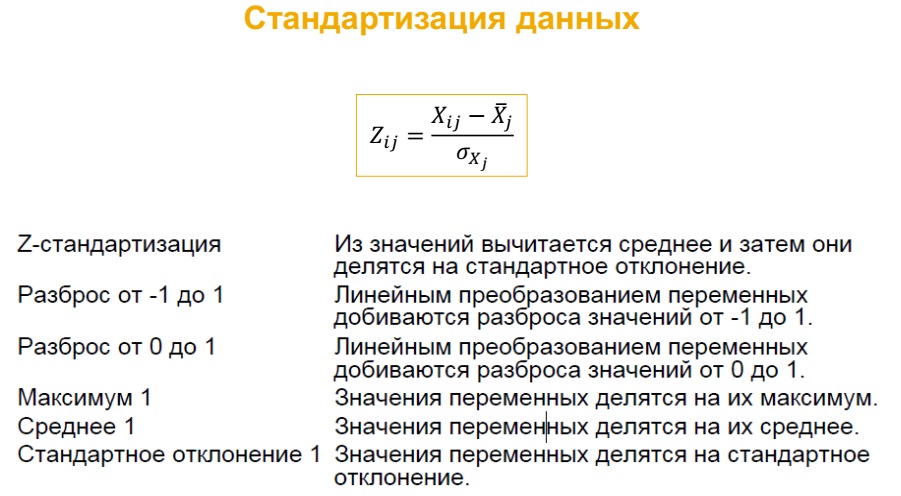
\includegraphics[scale=0.4]{images/lec07-pic24.png}
\end{figure}
\end{frame}

\begin{frame}{Расстояние между кластерами}
\begin{figure}[h]
\centering
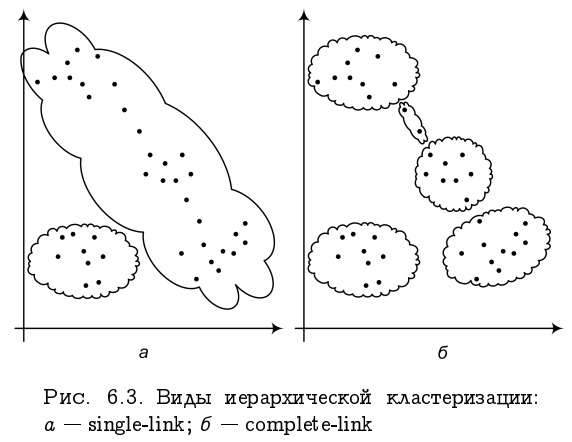
\includegraphics[scale=0.6]{images/lec07-pic18.png}
\end{figure}
\end{frame}

\section{Алгоритм кластеризации на основе теории графов}

\begin{frame}{Алгоритм кластеризации на основе теории графов}
\begin{figure}[h]
\centering
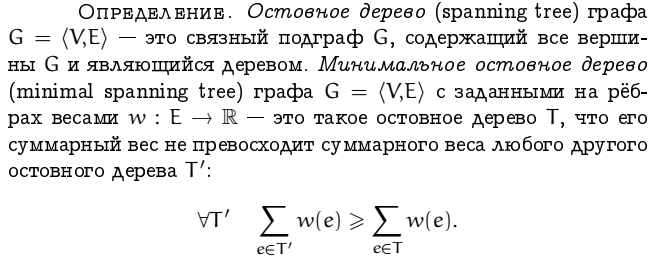
\includegraphics[scale=0.65]{images/lec07-pic19.png}
\end{figure}
\begin{enumerate}
\item построить минимальное остовное дерево;
\item выкидывать из него ребра максимального веса до тех пор, пока не получится нужное число кластеров. \end{enumerate}
Сколько ребер выбросим, столько кластеров получим.
\end{frame}

\begin{frame}{Алгоритм Краскала (Kruskal)}
\begin{figure}[h]
\centering
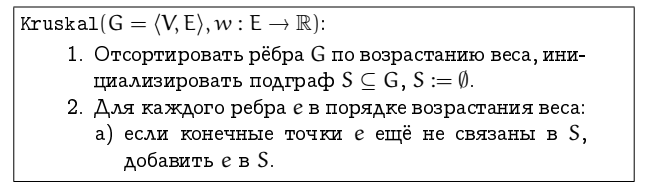
\includegraphics[scale=0.65]{images/lec07-pic20.png}
\end{figure}
\begin{enumerate}
\item на каждом шаге выбираем ребро с минимальным весом, 
\item если оно соединяет два дерева, добавляем его в остовное дерево, если нет, пропускаем. 
\end{enumerate}
\end{frame}

\begin{frame}{Алгоритм Борувски (Boruvka)}
\begin{figure}[h]
\centering
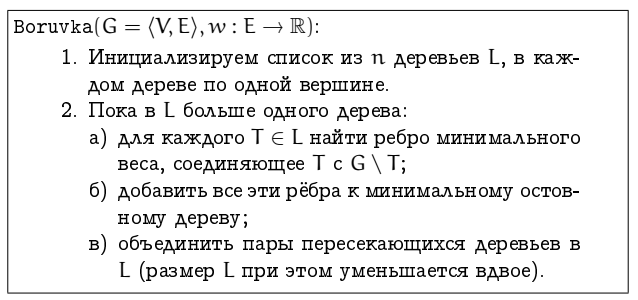
\includegraphics[scale=0.6]{images/lec07-pic21.png}
\end{figure}
\begin{enumerate}
\item можно строить минимальное остовное дерево, начав с одной вершины и добавляя ребра минимального
веса, пока не покроем весь граф (алгоритм Прима, Prim's algorithm);
\item будем делать то же самое, но во всех вершинах одновременно (распараллелим этот процесс).
\end{enumerate}
\end{frame}

\begin{frame}{Алгоритм k-средних (k-means)}
\begin{enumerate}
\item инициализировать центры кластеров каким-нибудь начальным разбиением; 
\item классифицировать точки по ближайшему к ним центру кластера;
\item перевычислить каждый из центров; 
\item если ничего не изменилось, остановиться, если изменилось  повторить.
\end{enumerate}
\begin{figure}[h]
\centering
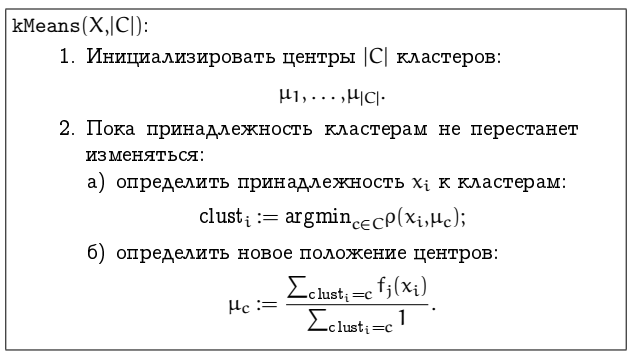
\includegraphics[scale=0.45]{images/lec07-pic22.png}
\end{figure}
\end{frame}

\begin{frame}{Алгоритм k-средних (k-means)}
\begin{figure}[h]
\centering
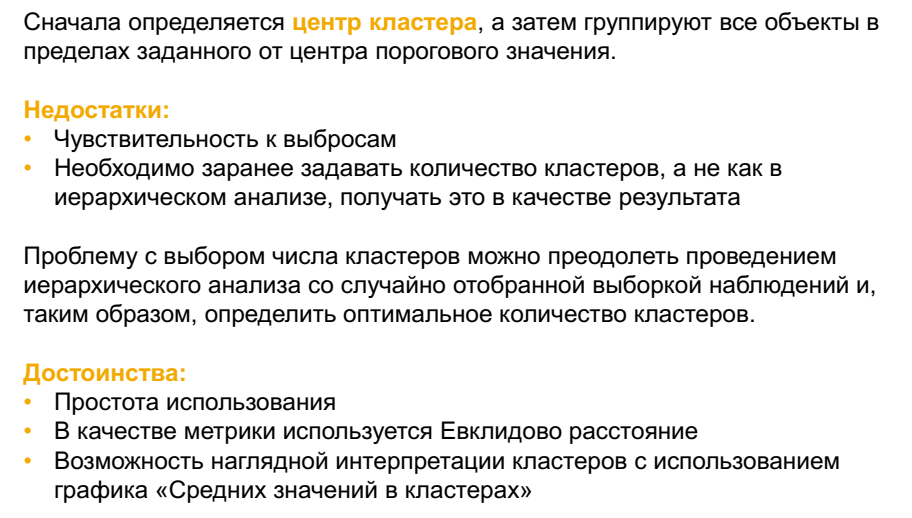
\includegraphics[scale=0.5]{images/lec07-pic23.png}
\end{figure}
\end{frame}

\begin{frame}{Пример некорретной кластеризации}
\begin{figure}[h]
\centering
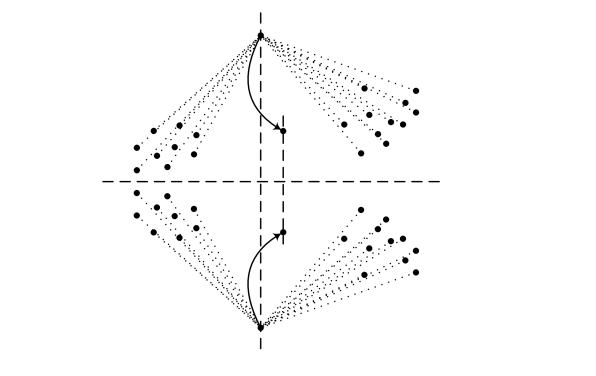
\includegraphics[scale=0.75]{images/lec07-pic25.png}
\end{figure}
\end{frame}

\section{Алгоритмы нечеткой кластеризации}

\begin{frame}{Алгоритмы нечеткой кластеризации}
\textbf{Мера принадлежности кластеру} - вещественное число из [0,1], и точки на краю кластера ѕменьше принадлежатї кластеру, чем в центре.

Будем обозначать принадлежность кластеру $c\in C$ через $u_c(x)$. Меры принадлежности обычно выбирают так, чтобы
\begin{figure}[h]
\centering
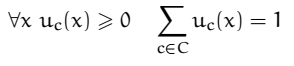
\includegraphics[scale=0.75]{images/lec07-pic29.png}
\end{figure}
Нечеткие алгоритмы кластеризации (одним из которых является алгоритм c-средних) минимизируют ту или иную меру ошибки. Часто применяется мера
\begin{figure}[h]
\centering
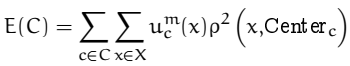
\includegraphics[scale=0.75]{images/lec07-pic30.png}
\end{figure}
где m - некоторый вещественный параметр.
\end{frame}

\begin{frame}{Алгоритмы нечеткой кластеризации}
\begin{figure}[h]
\centering
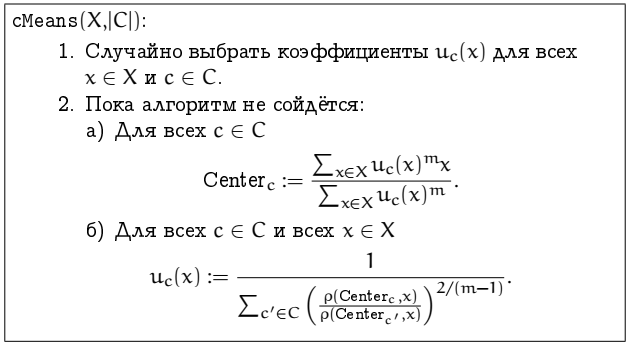
\includegraphics[scale=0.5]{images/lec07-pic31.png}
\end{figure}
\begin{itemize}
\item при $m=2$, то перевзвешивание эквивалентно линейной нормализации коэффициентов так, чтобы их сумма была равна единице. 
\item при $m\rightarrow 1$ все больший и больший вес придается самому близкому кластеру, и алгоритм становится все более похож на алгоритм k-средних.
\end{itemize}
\end{frame}

\begin{frame}{Этапы кластерного анализа}
\begin{figure}[h]
\centering
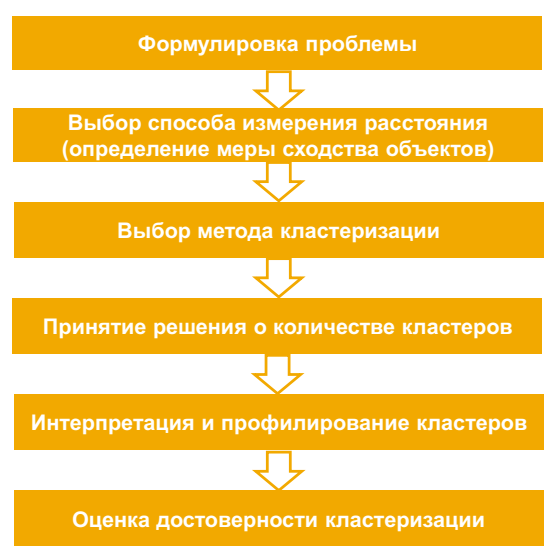
\includegraphics[scale=0.5]{images/lec07-pic28.png}
\end{figure}
\end{frame}

\begin{frame}{Принятие решений о числе кластеров}
\begin{figure}[h]
\centering
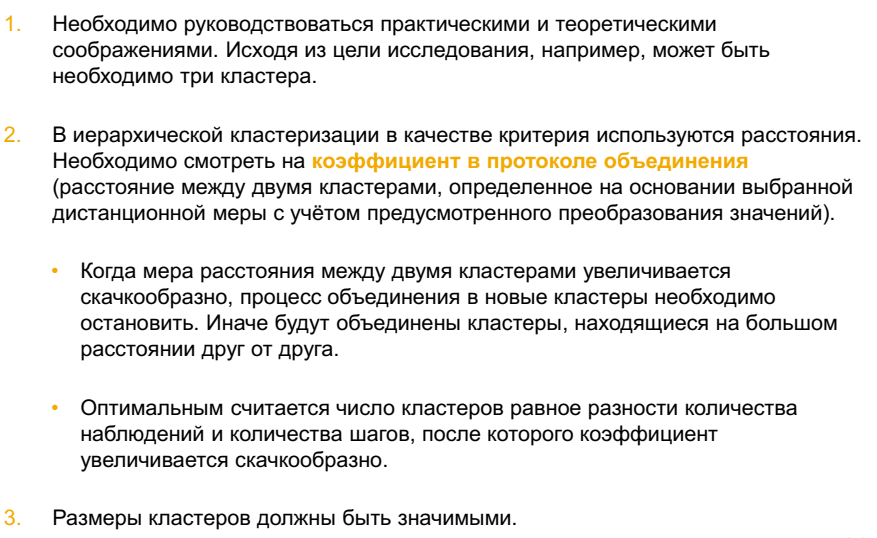
\includegraphics[scale=0.5]{images/lec07-pic26.png}
\end{figure}
\end{frame}

\begin{frame}{Оценка качества кластеризации}
\begin{figure}[h]
\centering
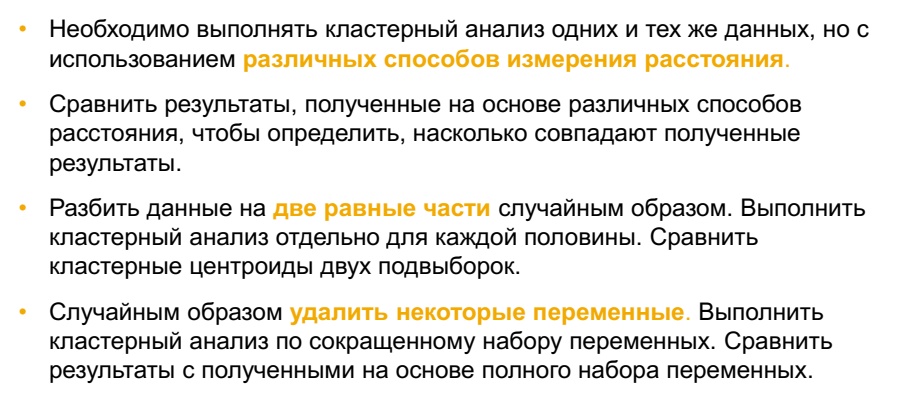
\includegraphics[scale=0.5]{images/lec07-pic27.png}
\end{figure}
\end{frame}

\section{Примеры проведения кластерного анализа}

\subsection{Пример 1}

\begin{frame}{Пример 1. Тестирование алгоритма k-means}
Исходный набор данных
\begin{figure}[h]
\centering
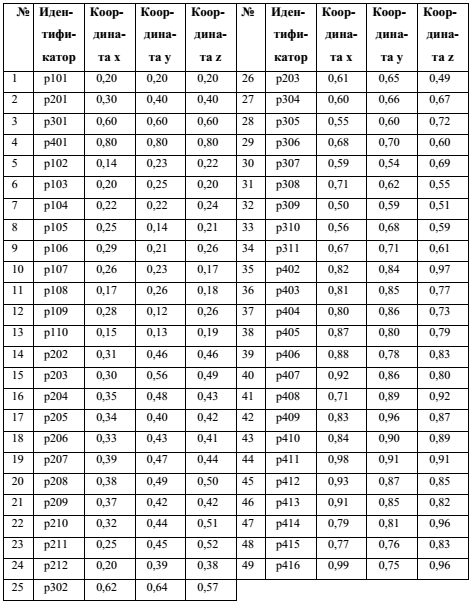
\includegraphics[scale=0.4]{images/lec07-pic32.png}
\end{figure}
\end{frame}

\begin{frame}{Пример 1. Тестирование алгоритма k-means}
Средние значения координат всей статистической совокупности
\begin{figure}[h]
\centering
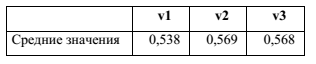
\includegraphics[scale=0.6]{images/lec07-pic33.png}
\end{figure}
Ковариационная матрица статистической совокупности
\begin{figure}[h]
\centering
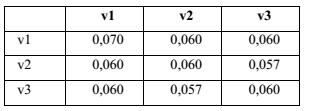
\includegraphics[scale=0.6]{images/lec07-pic34.png}
\end{figure}
Среднеквадратические отклонения 
\begin{figure}[h]
\centering
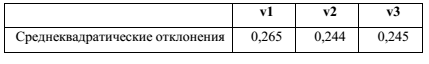
\includegraphics[scale=0.6]{images/lec07-pic35.png}
\end{figure}
\end{frame}

\begin{frame}{Пример 1. Тестирование алгоритма k-means}
Взаимное расположение данных в пространстве
\begin{figure}[h]
\centering
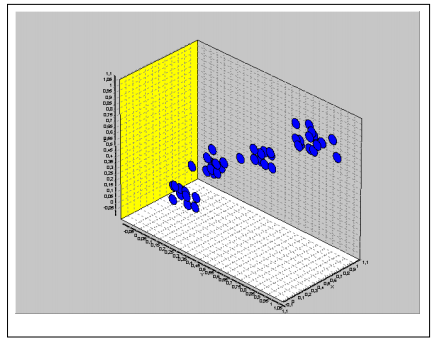
\includegraphics[scale=0.7]{images/lec07-pic36.png}
\end{figure}
\end{frame}

\begin{frame}{Пример 1. Тестирование алгоритма k-means}
Результаты работы алгоритма k-means
\begin{figure}[h]
\centering
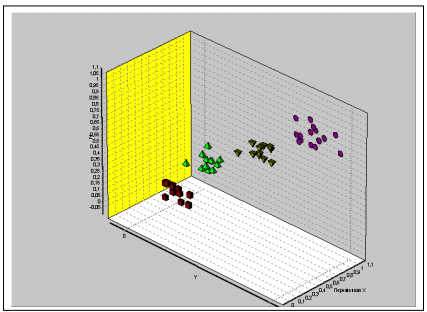
\includegraphics[scale=0.7]{images/lec07-pic37.png}
\end{figure}
\end{frame}

\begin{frame}{Пример 1. Тестирование алгоритма k-means}
Расстояния между кластерами
\begin{figure}[h]
\centering
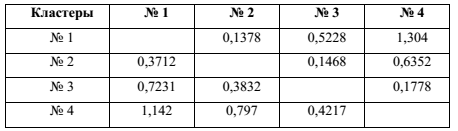
\includegraphics[scale=0.5]{images/lec07-pic38.png}
\end{figure}
Средние значения координат в кластерах
\begin{figure}[h]
\centering
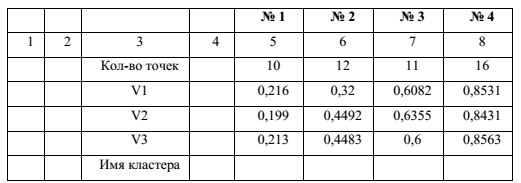
\includegraphics[scale=0.5]{images/lec07-pic39.png}
\end{figure}
\end{frame}

\begin{frame}{Пример 1. Тестирование алгоритма k-means}
Средние значения координат в кластерах
\begin{figure}[h]
\centering
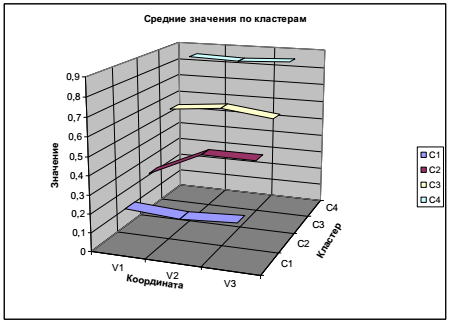
\includegraphics[scale=0.7]{images/lec07-pic40.png}
\end{figure}
\end{frame}

\begin{frame}{Пример 1. Тестирование алгоритма k-means}
Средние значения координат в кластерах
\begin{figure}[h]
\centering
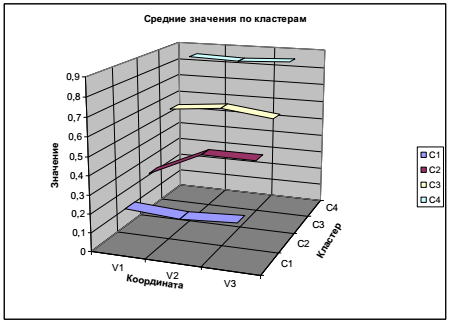
\includegraphics[scale=0.7]{images/lec07-pic40.png}
\end{figure}
\end{frame}

\begin{frame}{Пример 1. Тестирование алгоритма k-means}
Критерий Фишера проверки гипотезы о различии средних значений к кластерах
\begin{figure}[h]
\centering
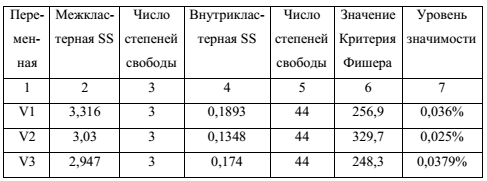
\includegraphics[scale=0.7]{images/lec07-pic41.png}
\end{figure}
\end{frame}

\subsection{Пример 2}

\begin{frame}{Пример 2. Исследование структуры личных подсобных хозяйств}
\begin{itemize}
\item В выборку вошли \textbf{29010} хозяйств Саратовской области.
\item Кластерный анализ проводился с помощью алгоритма k-средних.
\item Разбиение проводилось на 16, 24 и 32 кластера. 
\item Из множества показателей, содержащихся в переписном листе 3 ЛПХ, выделены 43 наиболее значимых
(по мнению экспертов) показателя. 
\end{itemize}
Условные названия групп показателей:
\begin{itemize}
\item А – трудовые ресурсы (показатели V1, V2);
\item В – площади земли (показатели V3..V6);
\item С – площади посевов (показатели V7..V12);
\item D – деревья, кусты и ягодники (показатели V13..V18);
\item Е – скот (показатели V19..V26, V32);
\item F – птица (показатели V27..V31);
\item G – места для содержания скота и птицы (показатели V33..V37);
\item H – техника (показатели V38..V43).
\end{itemize}
\end{frame}

\begin{frame}
Обозначение показателей
\begin{figure}[h]
\centering
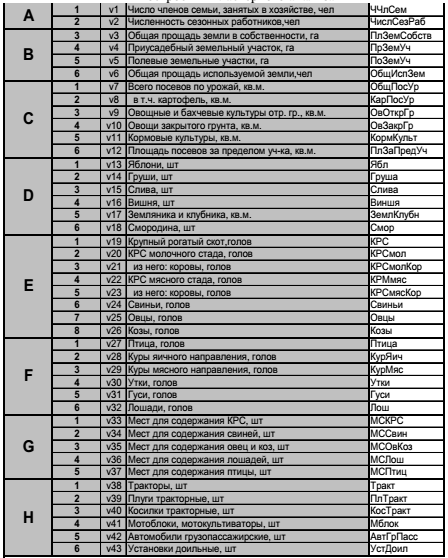
\includegraphics[scale=0.5]{images/lec07-pic42.png}
\end{figure}
\end{frame}

\begin{frame}
Кластеры и средние значения показателей
\begin{figure}[h]
\centering
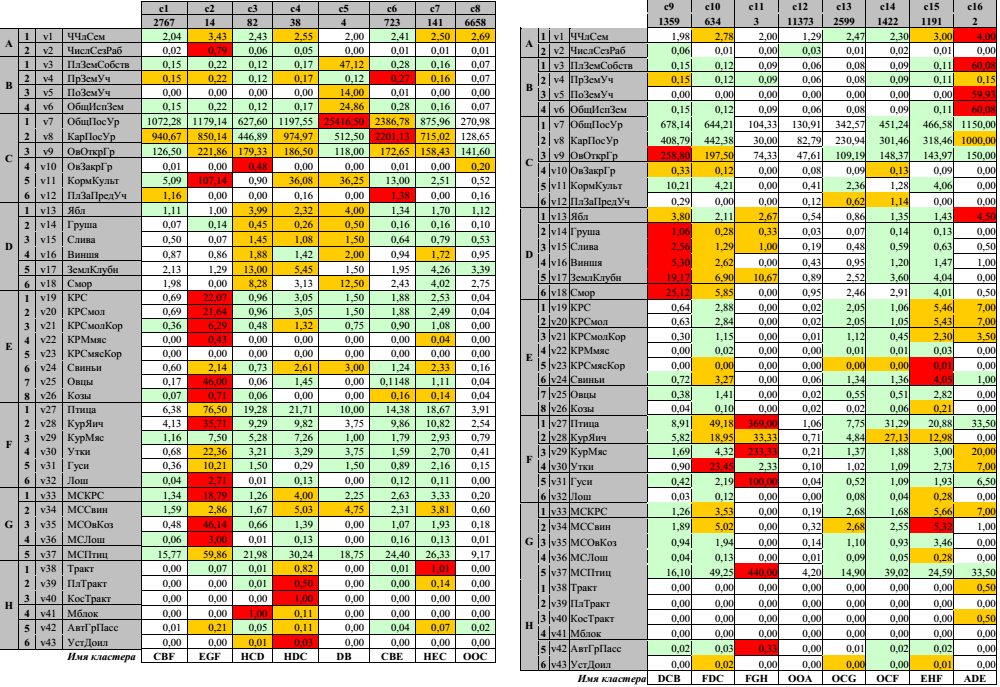
\includegraphics[scale=0.4]{images/lec07-pic43.png}
\end{figure}
\end{frame}

\begin{frame}
Кластеры и средние значения показателей
\begin{figure}[h]
\centering
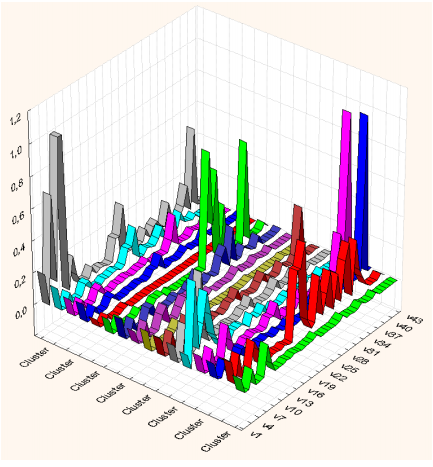
\includegraphics[scale=0.5]{images/lec07-pic44.png}
\end{figure}
\end{frame}

\begin{frame}
Кластеры и средние значения показателей
\begin{figure}[h]
\centering
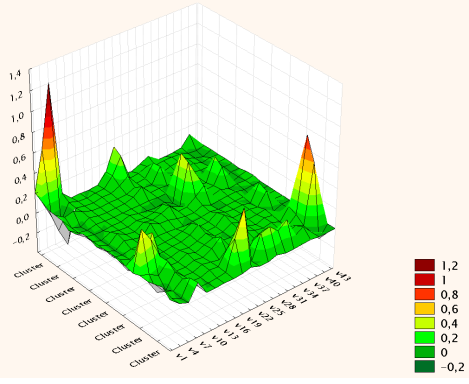
\includegraphics[scale=0.5]{images/lec07-pic45.png}
\end{figure}
\end{frame}

\begin{frame}
Сравнение разбиений с разным количеством показателей
\begin{figure}[h]
\centering
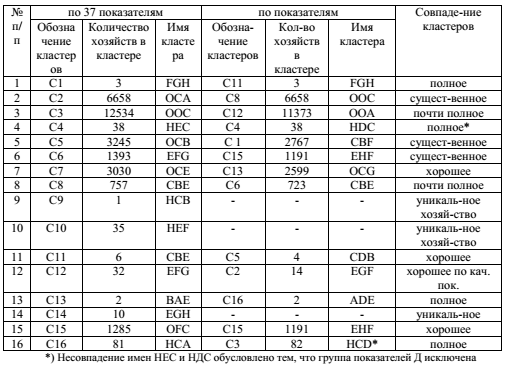
\includegraphics[scale=0.75]{images/lec07-pic46.png}
\end{figure}
\end{frame}

\end{document}